\documentclass[aspectratio=169]{beamer}

\usepackage[utf8]{inputenc}

\usepackage{color}
\usepackage{listings}
\usepackage{tikz}
\usepackage{hyperref}

\usetheme{Rochester}
\usecolortheme{beaver}

\addtobeamertemplate{navigation symbols}{}{%
    \usebeamerfont{footline}%
    \usebeamercolor[fg]{footline}%
    \hspace{1em}%
    \insertframenumber/\inserttotalframenumber
}

\lstloadlanguages{C++}
    \lstset{%
        language={C++},
        basicstyle=\ttfamily,
        keywordstyle=\color{blue},
        showstringspaces=false,
        escapechar={§},
        escapeinside=||
    }

\newif\iftransitions
 \transitionstrue


\newif\iffast
% \fasttrue

\title{Type Punning Done Right}
%\subtitle{Lua for C++ Programmers}
\author{Andreas Weis}
\institute{BMW AG}
\date{MUC++, December 12, 2018}
%\titlegraphic{
\includegraphics[height=.25\textheight]{resources/cppcon.png}}


\begin{document}

\frame{\titlepage}


\begin{frame}[fragile]
  \frametitle{What is type punning?}

  \iftransitions \pause \fi

  Accessing data through a pointer of unrelated type. \\[2ex]

  \iftransitions \pause \fi
   
  The act of type punning itself does not change the underlying data.
  
  It controls the \emph{operations} applied to that data.
\end{frame}


\begin{frame}[fragile]
  \frametitle{Types control operations}
  \setlength{\tabcolsep}{12pt}
  \begin{columns}
    \column{0.4\linewidth}
 
    \begin{lstlisting}
void increment(float& f) {
    ++f;
}

void increment(int& i) {
    ++i;
}
    \end{lstlisting}
    \iftransitions \pause \fi
    \column{0.5\linewidth}
    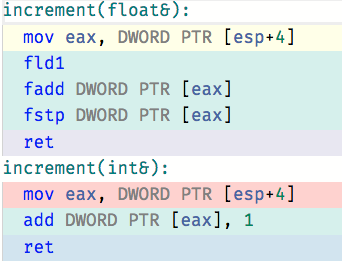
\includegraphics[height=.8\textheight]{resources/increment_float_int.png}
  \end{columns}
\end{frame}


\begin{frame}[fragile]

  \frametitle{Sometimes we actually want a different operation}
  
  \begin{lstlisting}
void add_ulp(float& f)
{
  (*(int*)(&f))++;    // here be dragons!
}
  \end{lstlisting}
\end{frame}

\begin{frame}
  \frametitle{This is technically incorrect in both C and C++.}

  \begin{center}
  
\includegraphics[height=.9\textheight]{resources/technically_incorrect.jpg}
  \end{center}
\end{frame}


\begin{frame}[fragile]
  \frametitle{Aliasing}

  \iftransitions \pause \fi

  % Aliasing is when the same thing is accessed through different names.

  % \iftransitions \pause \fi

  \begin{lstlisting}
void foo(int* a, int* b) {
  *a = 1;
  *b = 2;
}
  \end{lstlisting}
  \iftransitions \pause \fi
  \begin{lstlisting}
int x;
foo(&x, &x);
  \end{lstlisting}

%  \iftransitions \pause \fi

%  Aliasing forces the compiler to respect a corner case that is unlikely to ever occur in practice.

%  Fortran does not allow aliasing in this case and might thus be able to generate faster code here.

%  C99 introduced the \texttt{restrict} keyword to indicate alias-free pointers.
\end{frame}


\begin{frame}[fragile]
  \frametitle{Strict Aliasing in C and C++}

  % Type-based aliasing: If two pointers have different types, they must not alias.

  % \iftransitions \pause \fi
  
  \begin{lstlisting}
void bar(int* a, float* b)
{
  *a = 1;
  *b = 2.f;
}
  \end{lstlisting}
  \begin{lstlisting}
int x;
foo(&x, reinterpret_cast<float*>(&x));  // undefined behavior
  \end{lstlisting}
  
%  Effectively makes na\"ive type punning illegal.
\end{frame}



\begin{frame}[fragile]
  \frametitle{Type punning done right}

  \iftransitions
  \setbeamercolor{alerted text}{fg=red}
  \setbeamerfont{alerted text}{series=\bfseries,family=\ttfamily}
  \begin{semiverbatim}
\uncover<1->{\alert<0>{{\color{blue}void} add_ulp({\color{blue}float}& f)}}
\uncover<1->{\alert<0>{\{}}
\uncover<3->{\alert<0>{    {\color{blue}static_assert}({\color{blue}sizeof}({\color{blue}float}) == {\color{blue}sizeof}(uint32_t));}}
\uncover<2->{\alert<0>{    uint32_t tmp;}}
\uncover<4->{\alert<0>{    memcpy(&tmp, &f, {\color{blue}sizeof}({\color{blue}float}));}}
\uncover<2->{\alert<0>{    ++tmp;}}
\uncover<4->{\alert<0>{    memcpy(&f, &tmp, {\color{blue}sizeof}({\color{blue}float}));}}
\uncover<1->{\alert<0>{\}}}
  \end{semiverbatim}
  \else
  
  \begin{lstlisting}
void add_ulp(float& f)
{
    static_assert(sizeof(float) == sizeof(uint32_t));
    uint32_t tmp;
    memcpy(&tmp, &f, sizeof(float));
    ++tmp;
    memcpy(&f, &tmp, sizeof(float));
}
  \end{lstlisting}
  \fi
  
  \iftransitions \uncover<5->{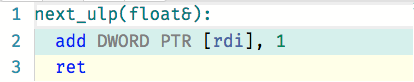
\includegraphics[height=.2\textheight]{resources/ulp_memcpy.png}} \else 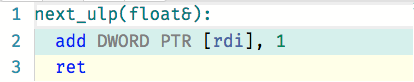
\includegraphics[height=.2\textheight]{resources/ulp_memcpy.png} \fi

\end{frame}


\begin{frame}[fragile]
  \frametitle{Goal: Don't lie to the compiler!}
\end{frame}

\begin{frame}
  \frametitle{If you want to know more...}

  \begin{itemize}
  \item CppCon 2017: \emph{Scott Schurr - Type Punning in C++17: Avoiding Pun-defined Behavior} \\ \href{https://www.youtube.com/watch?v=sCjZuvtJd-k}{https://www.youtube.com/watch?v=sCjZuvtJd-k}
  \end{itemize}
    
\end{frame}

\begin{frame}
  \frametitle{Thanks for your attention.}
  \begin{itemize}
    \setlength\itemsep{1.5em}

    \item \href{https://stackoverflow.com/users/577603/comicsansms}{
\includegraphics[height=.05\textheight]{resources/so-icon.png}} \href{https://github.com/ComicSansMS}{
\includegraphics[height=.05\textheight]{resources/github-icon.png}} 
\includegraphics[height=.05\textheight]{resources/slack-icon.png} ComicSansMS

    \item \href{https://twitter.com/DerGhulbus/}{
\includegraphics[height=.05\textheight]{resources/twitter-icon.png} @DerGhulbus}

  \end{itemize}

\end{frame}


\end{document}
